\documentclass[aspectratio=169,10pt]{beamer}

% ============================== THEME & FONTS ==============================
\usefonttheme{serif}
\useinnertheme[shadow=true]{rounded}

% ============================== PACKAGES ============================
\usepackage[utf8]{inputenc}
\usepackage[T1]{fontenc}
\usepackage{lmodern}
\usepackage{booktabs}
\usepackage{tabularx}
\usepackage{array}
\usepackage{graphicx}
\usepackage{amsmath,amssymb}
\usepackage{tikz}
\usetikzlibrary{arrows.meta, positioning, shapes.geometric, fit, backgrounds, calc, decorations.pathreplacing, trees}
\usepackage{pgfplots}
\pgfplotsset{compat=1.17}
\usepackage{xcolor}
\usepackage{multirow}
\usepackage{textpos}

% ============================== EXACT PALETTE ==============================
% Extracted directly from reference presentation:
\definecolor{mainblue}{rgb}{0.0, 0.2, 0.4}          % #003366 Deep Navy Blue
\definecolor{blockheaderblue}{rgb}{0.0, 0.3, 0.6}   % #004d99 Medium Dark Blue
\definecolor{blockbodyblue}{rgb}{0.9, 0.93, 0.96}   % #e6edf5 Soft Ice Blue tint
\definecolor{accentblue}{rgb}{0.0, 0.4, 0.8}       % #0066cc Bright Accent Blue
\definecolor{alertbodygray}{rgb}{0.941, 0.941, 0.941} % #f0f0f0 Light Gray
\definecolor{mutedblue}{rgb}{0.35, 0.48, 0.61}      % #597a9c Steel Muted Blue

% Compatibility aliases for diagrams in presentation
\definecolor{navy}{rgb}{0.0, 0.2, 0.4}              % #003366
\definecolor{teal}{rgb}{0.0, 0.4, 0.8}              % #0066cc
\definecolor{orangeaccent}{rgb}{0.0, 0.4, 0.8}      % #0066cc
\definecolor{grayaccent}{rgb}{0.5, 0.5, 0.5}
\definecolor{redaccent}{rgb}{0.8, 0.2, 0.2}

% ============================== BEAMER STYLING ==============================
\setbeamercolor{title}{bg=mainblue,fg=white}
\setbeamercolor{subtitle}{fg=white}
\setbeamercolor{frametitle}{bg=mainblue,fg=white}
\setbeamercolor{structure}{fg=mainblue}
\setbeamercolor{alerted text}{fg=accentblue}

% Blocks: rounded with drop shadow
\setbeamercolor{block title}{bg=blockheaderblue,fg=white}
\setbeamercolor{block body}{bg=blockbodyblue,fg=black}
\setbeamercolor{block title alerted}{bg=accentblue,fg=white}
\setbeamercolor{block body alerted}{bg=alertbodygray,fg=black}
\setbeamercolor{block title example}{bg=accentblue,fg=white}
\setbeamercolor{block body example}{bg=alertbodygray,fg=black}

% Lists: circles and numbers in mainblue
\setbeamertemplate{itemize items}[circle]
\setbeamercolor{itemize item}{fg=mainblue}
\setbeamercolor{itemize subitem}{fg=mainblue}
\setbeamercolor{itemize subsubitem}{fg=mainblue}
\setbeamertemplate{enumerate items}[default]
\setbeamercolor{enumerate item}{fg=mainblue}
\setbeamercolor{enumerate subitem}{fg=mainblue}
\setbeamercolor{enumerate subsubitem}{fg=mainblue}

% Table of Contents: 3D sphere balls
\setbeamertemplate{sections/subsections in toc}[ball]
\setbeamercolor{section number projected}{bg=mainblue,fg=white}

% Frametitle: solid top banner
\setbeamertemplate{frametitle}{%
  \nointerlineskip%
  \begin{beamercolorbox}[wd=\paperwidth,ht=25pt,dp=6pt,leftskip=8.5pt]{frametitle}%
    \usebeamerfont{frametitle}\insertframetitle\par%
  \end{beamercolorbox}%
}

% Author separator: line break to stack authors cleanly like reference slide 1
\makeatletter
\def\beamer@andtitle{\\[4pt]}
\makeatother

\pdfstringdefDisableCommands{\def\translate#1{#1}}

% Title page: rounded shadow box for title/subtitle, authors and details centered below
\setbeamertemplate{title page}{%
  \vbox{}
  \vskip 1.2em%
  \begin{beamercolorbox}[sep=8pt,center,rounded=true,shadow=true]{title}%
    {\usebeamerfont{title}\bfseries\inserttitle\par}%
    \ifx\insertsubtitle\@empty\else%
      \vskip 0.4em%
      {\usebeamerfont{subtitle}\insertsubtitle\par}%
    \fi%
  \end{beamercolorbox}%
  \vskip 1.3em%
  \begin{centering}%
    {\usebeamerfont{author}\insertauthor\par}%
    \vskip 1.1em%
    {\usebeamerfont{institute}\footnotesize\insertinstitute\par}%
    \vskip 1.1em%
    {\usebeamerfont{date}\insertdate\par}%
  \end{centering}%
  \vfill%
}

% Footline: minimal, only slide numbers at bottom right
\setbeamertemplate{navigation symbols}{}
\setbeamertemplate{footline}{%
  \hfill%
  \usebeamercolor[fg]{page number in head/foot}%
  \usebeamerfont{page number in head/foot}%
  \tiny\insertframenumber{} / \inserttotalframenumber%
  \hspace*{8.5pt}\vskip5pt%
}

% Bibliography styling matching reference
\setbeamertemplate{bibliography item}[article]
\setbeamercolor{bibliography entry author}{fg=mainblue}
\setbeamercolor{bibliography entry title}{fg=black}
\setbeamercolor{bibliography entry location}{fg=mutedblue}
\setbeamercolor{bibliography entry note}{fg=mutedblue}

% ============================== INFO ================================
\title{Generalizable Decision-Making for CAVs at Unsignalized Intersections}
\subtitle{A Deep Reinforcement Learning Approach --- Baseline Reproduction \& Path to Generalization}
\author{Mahmudul Hasan (220041231) \and Ishmam Tahmid (220041259) \and Farhan Tahsin Khan (220041229)}
\institute{
    CSE 4610: Design Project \\[2pt]
    \small Supervisors: Ashraful Alam Khan \quad \& \quad Tanjila Alam Sathi \\
    \small Course Coordinator: Dr.\ Md.\ Azam Hossain
}
\date{September 14, 2026}

\begin{document}

% ============================== TITLE ==============================
\begin{frame}
	\titlepage
\end{frame}

\begin{frame}{Outline}
	\tableofcontents[hideallsubsections]
\end{frame}

% =====================================================================
\section{Introduction}
% =====================================================================

\subsection{The Problem}

\begin{frame}{The Problem}
	\centering
	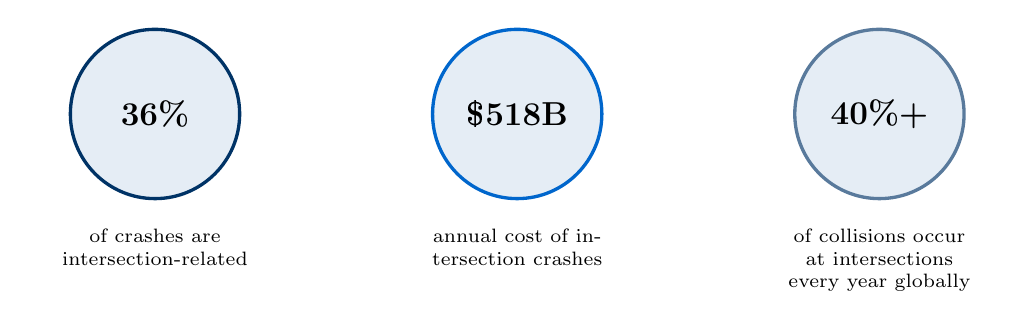
\begin{tikzpicture}[
			stat/.style={circle, draw=navy, very thick, fill=blockbodyblue, minimum size=2.15cm, align=center, font=\bfseries\large},
			lbl/.style={font=\scriptsize, text width=3.0cm, align=center}
		]
		\node[stat] (s1) at (0,0) {36\%};
		\node[stat, draw=accentblue] (s2) at (4.6,0) {\$518B};
		\node[stat, draw=mutedblue] (s3) at (9.2,0) {40\%+};
		\node[lbl, below=7pt of s1] {of crashes are intersection-related};
		\node[lbl, below=7pt of s2] {annual cost of intersection crashes};
		\node[lbl, below=7pt of s3] {of collisions occur at intersections every year globally};
	\end{tikzpicture}
	\vspace{18pt}
	\begin{columns}[T]
		\begin{column}{0.5\textwidth}
			\begin{itemize}
				\item Traffic lights control at the lane-group level, not per vehicle
				\item Fixed timing $\to$ stopping even when the road is clear
			\end{itemize}
		\end{column}
		\begin{column}{0.5\textwidth}
			\begin{itemize}
				\item Unsignalized crossings: high risk from occlusion \& uncertain intent
				\item No shared protocol $\to$ right-of-way must be inferred
			\end{itemize}
		\end{column}
	\end{columns}
\end{frame}

\subsection{Motivation}

\begin{frame}{Motivation: AV vs.\ CAV}
	\centering
	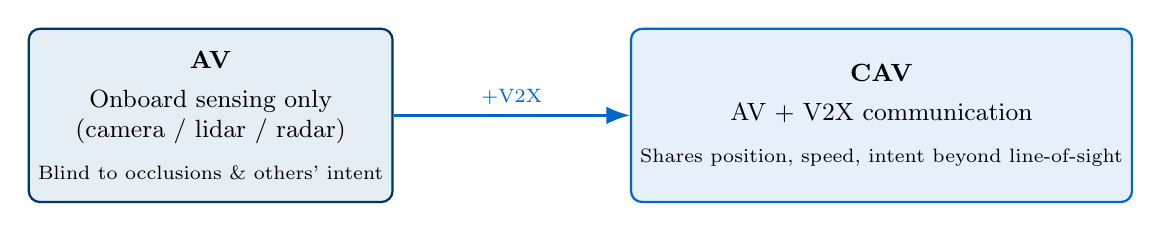
\begin{tikzpicture}[
			veh/.style={draw=navy, thick, rounded corners, fill=blockbodyblue, minimum width=4.6cm, minimum height=2.2cm, align=center, font=\small},
			arrowstyle/.style={-{Latex[length=3mm]}, thick, accentblue}
		]
		\node[veh] (av) {\textbf{AV}\\[3pt] Onboard sensing only\\(camera / lidar / radar)\\[4pt]\scriptsize Blind to occlusions \& others' intent};
		\node[veh, right=3.0cm of av, draw=accentblue, fill=accentblue!10] (cav) {\textbf{CAV}\\[3pt] AV + V2X communication\\[4pt]\scriptsize Shares position, speed, intent beyond line-of-sight};
		\draw[arrowstyle] (av) -- node[above, font=\scriptsize]{+V2X} (cav);
	\end{tikzpicture}
	\vspace{16pt}
	\begin{columns}[T]
		\begin{column}{0.5\textwidth}
			\begin{block}{Signal-Free AIM}
				\small Individual, continuous negotiation replaces group-level stopping
			\end{block}
		\end{column}
		\begin{column}{0.5\textwidth}
			\begin{block}{Deep RL}
				\small Learns adaptive go/yield behavior under stochastic traffic
			\end{block}
		\end{column}
	\end{columns}
	\vspace{8pt}

\end{frame}

\begin{frame}{Main Research Problem: Generalizable Decision-Making}
	\vspace{-4pt}
	\centering
	\textbf{\small Core Question: How can an autonomous vehicle make safe crossing decisions that \alert{generalize across arbitrary, unseen intersection topologies} without retraining?}\\[4pt]
	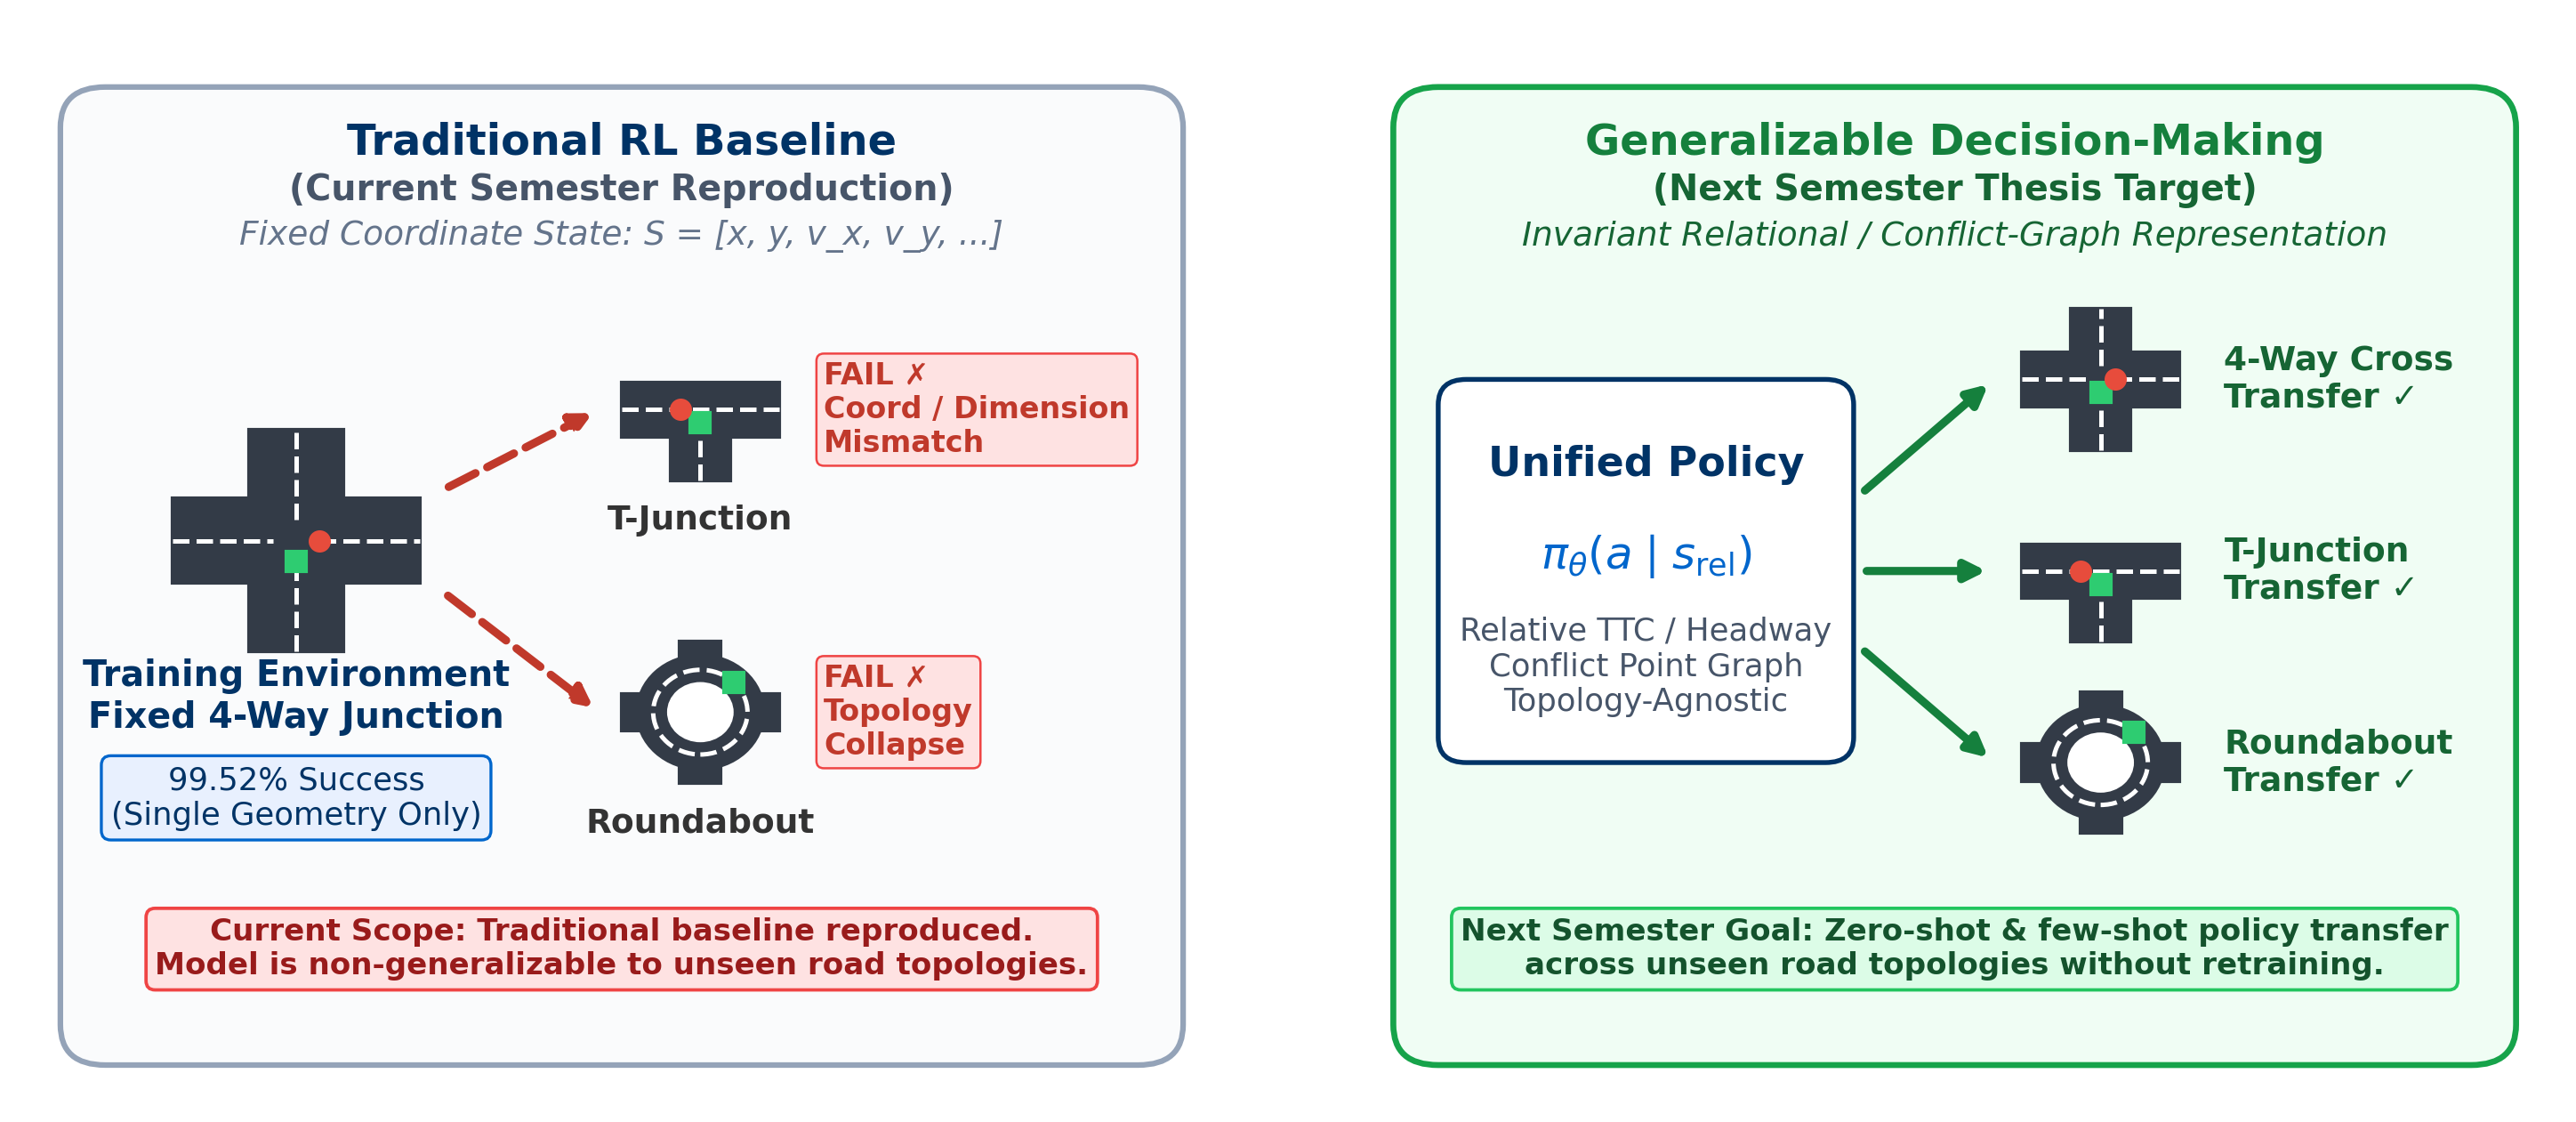
\includegraphics[width=0.88\linewidth]{img/generalizable_decision_concept.png}\\[4pt]
	\scriptsize
	\begin{columns}[T]
		\begin{column}{0.50\textwidth}
			\textbf{\color{navy}Current Semester (Completed):} Reproduced traditional RL baseline (fixed 4-way); demonstrated that single-geometry models \alert{do not generalize}.
		\end{column}
		\begin{column}{0.50\textwidth}
			\textbf{\color{accentblue}Next Semester (Thesis Goal):} Develop topology-invariant relational representations to achieve \textbf{zero-shot policy transfer} across unseen layouts.
		\end{column}
	\end{columns}
\end{frame}

\begin{frame}{Key Objectives}
	\begin{columns}
		\begin{column}{0.32\textwidth}
			\begin{block}{Safety}
				\centering \small
				Near-zero collisions across randomized, dense turning maneuvers.
			\end{block}
		\end{column}
		\begin{column}{0.32\textwidth}
			\begin{block}{Efficiency}
				\centering \small
				Maximize crossing speed and throughput without signal delays.
			\end{block}
		\end{column}
		\begin{column}{0.32\textwidth}
			\begin{block}{Generalizability}
				\centering \small
				Zero-/few-shot policy transfer across unseen geometries (Next Sem.).
			\end{block}
		\end{column}
	\end{columns}
\end{frame}

% =====================================================================
\section{Related Work}
% =====================================================================

\begin{frame}{Taxonomy of Coordination Strategies}
	\centering
	\resizebox{0.98\textwidth}{!}{%
		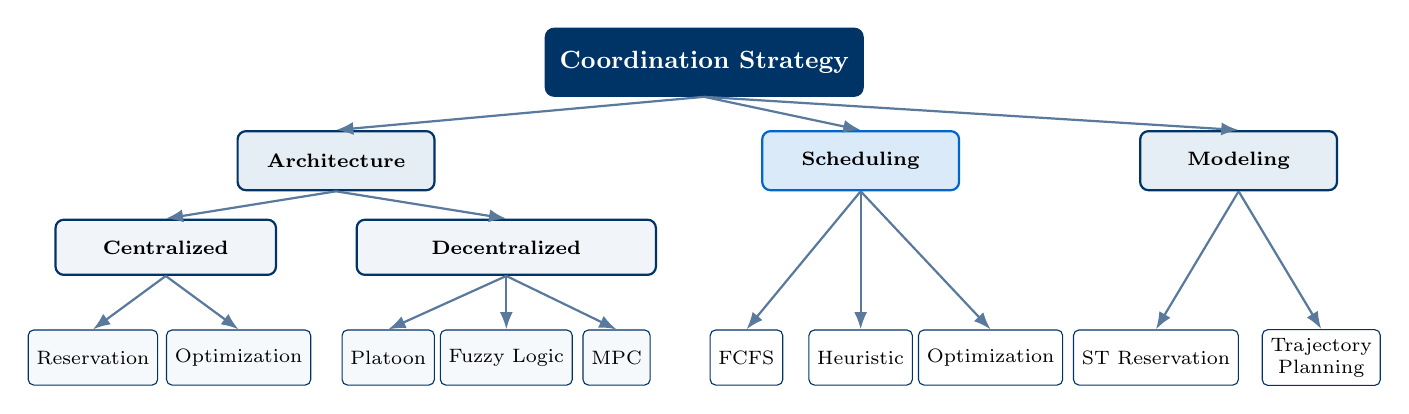
\begin{tikzpicture}[
				root/.style={fill=navy, text=white, font=\bfseries\small, draw=navy, thick, rounded corners=3pt, inner sep=5pt, minimum height=8.5mm},
				lvl1/.style={fill=blockbodyblue, font=\bfseries\scriptsize, draw=navy, thick, rounded corners=3pt, minimum width=2.5cm, minimum height=7.5mm},
				lvl1_accent/.style={fill=accentblue!14, font=\bfseries\scriptsize, draw=accentblue, thick, rounded corners=3pt, minimum width=2.5cm, minimum height=7.5mm},
				branch/.style={fill=blockbodyblue!55, font=\scriptsize\bfseries, draw=navy, thick, rounded corners=3pt, minimum height=7mm, align=center},
				leaf/.style={fill=white, font=\scriptsize, draw=navy, rounded corners=2pt, minimum height=7mm, inner sep=3pt, align=center},
				leaf_sub/.style={fill=blockbodyblue!35, font=\scriptsize, draw=navy, rounded corners=2pt, minimum height=7mm, inner sep=3pt, align=center},
				arrowstyle/.style={-{Latex[length=2.2mm]}, thick, mutedblue}
			]
			% --- Leaves across the bottom (y = -3.4) ---
			% Under Centralized (2)
			\node[leaf_sub] (c_res) at (0.85, -3.4) {Reservation};
			\node[leaf_sub] (c_opt) at (2.70, -3.4) {Optimization};

			% Under Decentralized (3)
			\node[leaf_sub] (d_plt) at (4.60, -3.4) {Platoon};
			\node[leaf_sub] (d_fuz) at (6.10, -3.4) {Fuzzy Logic};
			\node[leaf_sub] (d_mpc) at (7.50, -3.4) {MPC};

			% Under Scheduling (3)
			\node[leaf] (s_fcfs) at (9.15, -3.4) {FCFS};
			\node[leaf] (s_heur) at (10.60, -3.4) {Heuristic};
			\node[leaf] (s_opt) at (12.25, -3.4) {Optimization};

			% Under Modeling (2)
			\node[leaf] (m_st) at (14.35, -3.4) {ST Reservation};
			\node[leaf] (m_tp) at (16.45, -3.4) {Trajectory\\Planning};

			% --- Level 2 Intermediate Branches (y = -2.0) ---
			\path (c_res.north) -- (c_opt.north) coordinate[midway] (c_mid);
			\node[branch, minimum width=2.8cm] (central) at (c_mid |- 0,-2.0) {Centralized};

			\node[branch, minimum width=3.8cm] (decentral) at (d_fuz.north |- 0,-2.0) {Decentralized};

			% --- Level 1 Main Pillars (y = -0.9) ---
			\path (central.north) -- (decentral.north) coordinate[midway] (arch_mid);
			\node[lvl1] (arch) at (arch_mid |- 0,-0.9) {Architecture};

			\node[lvl1_accent] (sched) at (s_heur.north |- 0,-0.9) {Scheduling};

			\path (m_st.north) -- (m_tp.north) coordinate[midway] (mod_mid);
			\node[lvl1] (model) at (mod_mid |- 0,-0.9) {Modeling};

			% --- Root Node (y = 0.35) ---
			\path (c_res.west) -- (m_tp.east) coordinate[midway] (tree_center);
			\node[root] (root) at (tree_center |- 0, 0.35) {Coordination Strategy};

			% --- Connections ---
			\draw[arrowstyle] (root.south) -- (arch.north);
			\draw[arrowstyle] (root.south) -- (sched.north);
			\draw[arrowstyle] (root.south) -- (model.north);

			\draw[arrowstyle] (arch.south) -- (central.north);
			\draw[arrowstyle] (arch.south) -- (decentral.north);

			\draw[arrowstyle] (central.south) -- (c_res.north);
			\draw[arrowstyle] (central.south) -- (c_opt.north);

			\draw[arrowstyle] (decentral.south) -- (d_plt.north);
			\draw[arrowstyle] (decentral.south) -- (d_fuz.north);
			\draw[arrowstyle] (decentral.south) -- (d_mpc.north);

			\draw[arrowstyle] (sched.south) -- (s_fcfs.north);
			\draw[arrowstyle] (sched.south) -- (s_heur.north);
			\draw[arrowstyle] (sched.south) -- (s_opt.north);

			\draw[arrowstyle] (model.south) -- (m_st.north);
			\draw[arrowstyle] (model.south) -- (m_tp.north);

		\end{tikzpicture}%
	}
	\vspace{8pt}
\end{frame}

\begin{frame}{What the Literature Shows}
	\centering
	\small
	\begin{tabular}{lll}
		\toprule
		\textbf{Axis} & \textbf{Most popular}      & \textbf{Runner-up}          \\
		\midrule
		Goal          & Safety + Efficiency (37\%) & Safety alone (26\%)         \\
		Architecture  & V2V (159 papers)           & V2I (119 papers)            \\
		Scheduling    & Optimization (277 papers)  & Heuristic (20 papers)       \\
		Modeling      & Trajectory Planning        & Spatio-Temporal Reservation \\
		\bottomrule
	\end{tabular}
	\vspace{14pt}


\end{frame}


\begin{frame}{RL Literature Thread I: Single-Ego Decision Making}
	\scriptsize
	\begin{table}
		\begin{tabularx}{\textwidth}{@{}l X X X@{}}
			\toprule
			\textbf{Paper}       & \textbf{Idea}                           & \textbf{Architecture}     & \textbf{Key finding}                \\
			\midrule
			Isele et al.\ (2018) & DQN vs.\ TTC + occlusion ``creeping''   & Single-agent, no comm.    & 28\% faster, $<$1\% collisions      \\
			Wu et al.\ (2019)    & Decentralized coordination Q-learning   & Multi-agent, sparse comm. & Beats FCFS/LQF/Webster              \\
			Kai et al.\ (2020)   & One policy, 3 maneuvers via task vector & Single-agent              & Matches/beats 3 separate DQNs       \\
			Shu et al.\ (2022)   & Weight transfer across maneuvers        & Single-agent              & Same-task 100\%, cross-task $>$70\% \\
			\bottomrule
		\end{tabularx}
	\end{table}
\end{frame}

\begin{frame}{RL Literature Thread II: Graph Representations \& Cooperative AIM}
	\scriptsize
	\begin{table}
		\begin{tabularx}{\textwidth}{@{}l X X@{}}
			\toprule
			\textbf{Paper}              & \textbf{Contribution}                                   & \textbf{Setting}                      \\
			\midrule
			Chen et al.\ (2025)         & Scenario-agnostic ``lane-gap'' + PPO + CILQR            & Single-ego, multi-scenario (93--97\%) \\
			Schier et al.\ (2023)       & Vehicle+road graph, learned edges                       & Predicts right-of-way at 99.5\% acc.  \\
			Klimke et al.\ (2022)       & Edge-augmented RGCN + TD3, controls \emph{all} vehicles & True cooperative AIM          \\
			Huamán Reyna et al.\ (2026) & Survey, 53 papers                                       & Hybrid methods score best overall     \\
			\bottomrule
		\end{tabularx}
	\end{table}
	\vspace{8pt}
	\begin{block}{Where we fit}
		\small
		\begin{itemize}
			\item Single-ego decision-making, multi-task state (like Kai et al., Xiao et al.)
			\item Not centralized AIM (Klimke et al.) --- tractable scope, still comparable
		\end{itemize}
	\end{block}
\end{frame}

% =====================================================================
\section{Methodology}
% =====================================================================

\begin{frame}{Methodology at a Glance}
	\centering
	\resizebox{\textwidth}{!}{%
		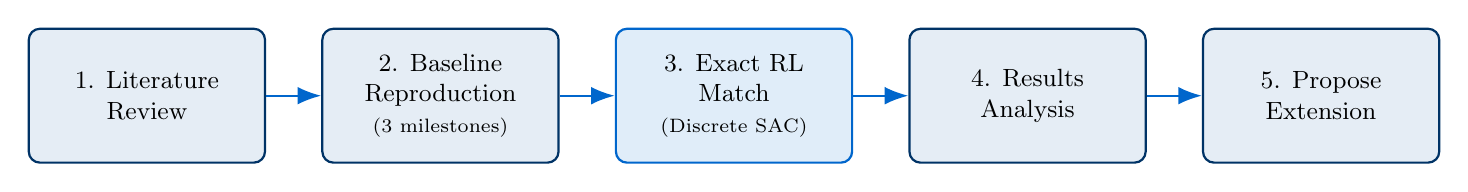
\begin{tikzpicture}[
				node distance=7mm,
				mstep/.style={draw=navy, thick, rounded corners, fill=blockbodyblue, minimum height=1.7cm, minimum width=3.0cm, align=center, font=\small},
				arrowstyle/.style={-{Latex[length=3mm]}, thick, accentblue}
			]
			\node[mstep] (a) {1. Literature\\Review};
			\node[mstep, right=of a] (b) {2. Baseline\\Reproduction\\\scriptsize (3 milestones)};
			\node[mstep, right=of b, fill=accentblue!12, draw=accentblue] (c) {3. Exact RL\\Match\\\scriptsize (Discrete SAC)};
			\node[mstep, right=of c] (d) {4. Results\\Analysis};
			\node[mstep, right=of d] (e) {5. Propose\\Extension};
			\draw[arrowstyle] (a) -- (b);
			\draw[arrowstyle] (b) -- (c);
			\draw[arrowstyle] (c) -- (d);
			\draw[arrowstyle] (d) -- (e);
		\end{tikzpicture}%
	}
	\vspace{14pt}
	\small Each stage builds on the previous milestone's validated pipeline --- detailed next.
\end{frame}

\begin{frame}{Reproduction Target: Xiao et al.\ (2024, IEEE T-VT)}
	\small \textbf{``Decision-Making for AVs in Random Task Scenarios at Unsignalized Intersection Using Deep RL''}
	\vspace{8pt}
	\begin{columns}[T]
		\begin{column}{0.52\textwidth}
			\textbf{Three contributions}
			\begin{enumerate}
				\item \textbf{Mix-Attention Network} (replaces plain MLP)
				\item \textbf{Task-intent variable} $\mu_a$
				\item \textbf{Segmented replay buffer}
			\end{enumerate}
		\end{column}
		\begin{column}{0.45\textwidth}
			\begin{block}{Setting}
				\small 4-way, single-lane, unsignalized; random task/episode; \texttt{highway-env}; Discrete SAC, 50{,}000 episodes
			\end{block}
		\end{column}
	\end{columns}
\end{frame}

\begin{frame}{Disclaimer: Scope of This Work}
	\begin{alertblock}{Reproduction \& benchmarking study --- not our primary contribution}
		\small Build a working pipeline, understand the environment deeply, then propose a novel direction.
	\end{alertblock}
	\vspace{10pt}
	\textbf{Acknowledged limitations}
	\begin{itemize}
		\item Original source code not released
		\item Some hyperparameters / reward constants only partially specified
		\item Reproduction is faithful, but not byte-for-byte
	\end{itemize}
\end{frame}

\begin{frame}{Research Progression: Three Milestones}
	\centering
	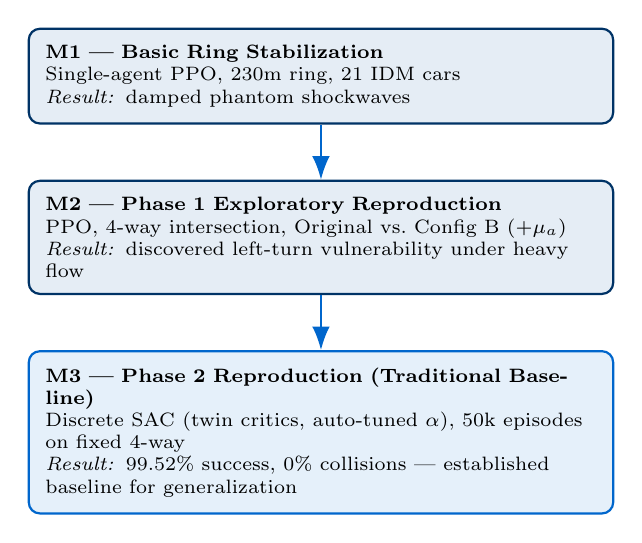
\begin{tikzpicture}[
			node distance=7mm and 14mm,
			every node/.style={font=\scriptsize},
			box/.style={draw=navy, thick, rounded corners, fill=blockbodyblue, text width=7cm, align=left, inner sep=6pt},
			arrowstyle/.style={-{Latex[length=3mm]}, thick, accentblue}
		]
		\node[box] (m1) {
			\textbf{M1 --- Basic Ring Stabilization}\\
			Single-agent PPO, 230m ring, 21 IDM cars\\
			\textit{Result:} damped phantom shockwaves
		};
		\node[box, below=of m1] (m2) {
			\textbf{M2 --- Phase 1 Exploratory Reproduction}\\
			PPO, 4-way intersection, Original vs.\ Config B ($+\mu_a$)\\
			\textit{Result:} discovered left-turn vulnerability under heavy flow
		};
		\node[box, below=of m2, fill=accentblue!10, draw=accentblue] (m3) {
			\textbf{M3 --- Phase 2 Reproduction (Traditional Baseline)}\\
			Discrete SAC (twin critics, auto-tuned $\alpha$), 50k episodes on fixed 4-way\\
			\textit{Result:} 99.52\% success, 0\% collisions --- established baseline for generalization
		};
		\draw[arrowstyle] (m1) -- (m2);
		\draw[arrowstyle] (m2) -- (m3);
	\end{tikzpicture}
\end{frame}

\begin{frame}{State Space Formulation}
	\small
	\vspace{-6pt}
	\centering
	\textbf{Observation vector} (48\,m radar radius, up to 9 nearest surrounding vehicles):\\
	\vspace{1pt}
	$\mathbf{S} = \big[\, S_{\text{ego}}, \; S_1, \; S_2, \; \dots, \; S_9 \,\big]$
	\vspace{2pt}

	\begin{columns}[T]
		\begin{column}{0.49\textwidth}
			\begin{block}{Ego Vehicle State ($S_{\text{ego}} \in \mathbb{R}^{6\text{ or }7}$)}
				\scriptsize
				$\mathbf{S_{\text{ego}}} = [\, p_{\text{ego}}, \; x, \; y, \; v_x, \; v_y, \; \phi, \; (\mu_a) \,]$
				\vspace{2pt}
				\begin{itemize}\setlength{\itemsep}{1.5pt}
					\item $p_{\text{ego}} \in \{0, 1\}$: \textbf{Existence flag} ($1 = \text{present}$)
					\item $x, y$: \textbf{Global position} coordinates (m)
					\item $v_x, v_y$: \textbf{Absolute velocity} along $x, y$ (m/s)
					\item $\phi$: \textbf{Heading angle} / orientation (rad)
					\item $\mu_a$: \textbf{Task-intent feature} (\textit{Config B only})\\
					      Encodes route (left/straight/right) \& exit progress
				\end{itemize}
			\end{block}
		\end{column}
		\begin{column}{0.49\textwidth}
			\begin{block}{9 Surrounding Vehicles ($S_i \in \mathbb{R}^{6}$ each)}
				\scriptsize
				$\mathbf{S_i} = [\, p_i, \; \Delta x_i, \; \Delta y_i, \; \Delta v_{x,i}, \; \Delta v_{y,i}, \; \phi_i \,]$
				\vspace{2pt}
				\begin{itemize}\setlength{\itemsep}{1.5pt}
					\item $p_i \in \{0, 1\}$: \textbf{Presence flag} ($0$ if empty / padded)
					\item $\Delta x_i, \Delta y_i$: \textbf{Relative position} $(x_i - x,\, y_i - y)$ (m)
					\item $\Delta v_{x,i}, \Delta v_{y,i}$: \textbf{Relative velocity} $(v_{x,i} - v_x,\, v_{y,i} - v_y)$ (m/s)
					\item $\phi_i$: \textbf{Heading angle} of vehicle $i$ (rad)
					\item \textbf{Ordering}: Sorted ascending by distance $d_i \le 48$\,m
				\end{itemize}
			\end{block}
		\end{column}
	\end{columns}
\end{frame}

\begin{frame}{Action Space \& Reward Function}
	\begin{columns}[T]
		\begin{column}{0.42\textwidth}
			\textbf{Action} (discrete, 3 values)
			\[
				A = \{\text{accel}, \text{idle}, \text{decel}\}
			\]
			\[
				a = K_{P,A}(v_{tar} - v), \;\; K_{P,A}=5
			\]
			\small Lateral control is a fixed PD controller --- RL controls only longitudinal speed.
		\end{column}
		\begin{column}{0.58\textwidth}
			\textbf{Reward}
			\[
				R = \begin{cases}
					+30  & \text{reach destination}  \\
					-120 & \text{collision}          \\
					+0.1 & \text{reach target speed}
				\end{cases}
			\]
			\begin{itemize}
				\item Sparse terminal terms (safety + completion)
				\item Small dense term rewards cruising
				\item Collision penalty $\gg$ arrival reward
			\end{itemize}
		\end{column}
	\end{columns}
\end{frame}

\begin{frame}{System Pipeline}
	\centering
	\resizebox{0.96\textwidth}{!}{%
		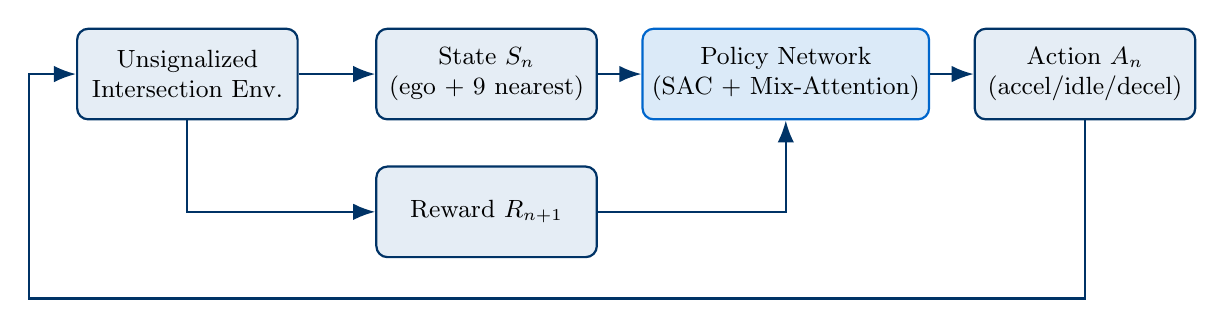
\begin{tikzpicture}[
				every node/.style={font=\small},
				block/.style={draw=navy, thick, rounded corners=4pt, fill=blockbodyblue, minimum height=1.15cm, minimum width=2.8cm, align=center},
				policyblock/.style={draw=accentblue, thick, rounded corners=4pt, fill=accentblue!14, minimum height=1.15cm, minimum width=2.8cm, align=center},
				arrowstyle/.style={-{Latex[length=2.8mm]}, thick, navy}
			]
			% Main row nodes
			\node[block] (env) at (0,0) {Unsignalized\\Intersection Env.};
			\node[block] (state) at (3.8,0) {State $S_n$\\(ego + 9 nearest)};
			\node[policyblock] (policy) at (7.6,0) {Policy Network\\(SAC + Mix-Attention)};
			\node[block] (action) at (11.4,0) {Action $A_n$\\(accel/idle/decel)};

			% Reward node: placed symmetrically below State
			\node[block] (reward) at (3.8,-1.75) {Reward $R_{n+1}$};

			% Forward arrows
			\draw[arrowstyle] (env.east) -- (state.west);
			\draw[arrowstyle] (state.east) -- (policy.west);
			\draw[arrowstyle] (policy.east) -- (action.west);

			% Symmetric Inner Reward loop: Env -> Reward -> Policy
			\draw[arrowstyle] (env.south) |- (reward.west);
			\draw[arrowstyle] (reward.east) -| (policy.south);

			% Outer Action-Environment feedback loop
			\coordinate (bot_y) at (0,-2.85);
			\coordinate (left_x) at ($(env.west)+(-0.6,0)$);

			\draw[arrowstyle] (action.south) -- (action.south |- bot_y)
			-- (left_x |- bot_y)
			|- (env.west);

		\end{tikzpicture}%
	}
\end{frame}

\begin{frame}{Discrete Soft Actor-Critic (Discrete SAC)}
	\small
	\begin{columns}[T]
		\begin{column}{0.48\textwidth}
			\textbf{Why SAC over PPO}
			\begin{itemize}
				\item Off-policy $\to$ sample efficient
				\item Max-entropy $\to$ broad exploration
				\item Auto-tuned $\alpha$ --- no fragile hyperparameter
			\end{itemize}
		\end{column}
		\begin{column}{0.52\textwidth}
			\[
				\pi^{*} = \arg\max_\pi \sum_{n} \mathbb{E}\big[\gamma^n (R_n + \alpha \mathcal{H}(\pi(\cdot|S_n)))\big]
			\]
			\begin{itemize}
				\item Twin Q-critics reduce overestimation bias
				\item Discrete policy: softmax over 3 actions
			\end{itemize}
		\end{column}
	\end{columns}
\end{frame}

% =====================================================================
\section{Implementation}
% =====================================================================

\begin{frame}{Implementation Stack}
	\centering
	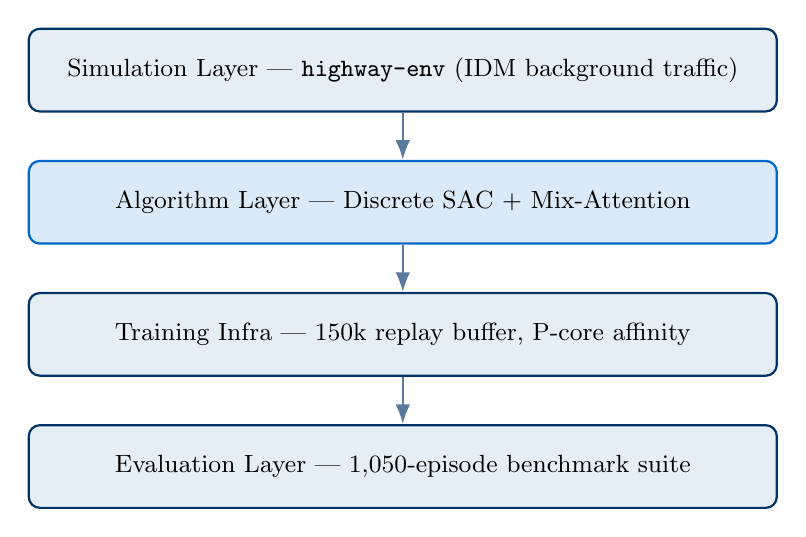
\begin{tikzpicture}[
			layer/.style={draw=navy, thick, rounded corners, minimum width=9.5cm, minimum height=1.05cm, align=center, font=\small},
			arrowstyle/.style={-{Latex[length=2.5mm]}, thick, mutedblue}
		]
		\node[layer, fill=blockbodyblue] (sim) {Simulation Layer --- \texttt{highway-env} (IDM background traffic)};
		\node[layer, fill=accentblue!14, draw=accentblue, below=6mm of sim] (algo) {Algorithm Layer --- Discrete SAC + Mix-Attention};
		\node[layer, fill=blockbodyblue, below=6mm of algo] (train) {Training Infra --- 150k replay buffer, P-core affinity};
		\node[layer, fill=blockbodyblue, below=6mm of train] (eval) {Evaluation Layer --- 1{,}050-episode benchmark suite};
		\draw[arrowstyle] (sim) -- (algo);
		\draw[arrowstyle] (algo) -- (train);
		\draw[arrowstyle] (train) -- (eval);
	\end{tikzpicture}
\end{frame}

\begin{frame}{Simulation \& Training Setup}
	\scriptsize
	\begin{table}
		\begin{tabularx}{\textwidth}{@{}l X X X X@{}}
			\toprule
			                & \textbf{Project 1: Ring}            & \textbf{Project 2: Phase 1} & \textbf{Project 3: Phase 2} & \textbf{Paper}        \\
			\midrule
			Scenario        & 230m ring                           & 4-way                       & 4-way                       & 4-way                 \\
			Sim.\ engine    & Flow + SUMO                         & Flow + SUMO                 & \texttt{highway-env}        & \texttt{highway-env}  \\
			Algorithm       & PPO                                 & PPO                         & \textbf{Discrete SAC}       & \textbf{Discrete SAC} \\
			Network         & Actor-Critic MLP                    & $[32,32,32]$                & $[256,256,64,3]$            & $[256,256,64,3]$      \\
			Obs.\ space     & 3-dim POMDP                         & 60 / 61-dim                 & 60 / 61-dim                 & 60 / 61-dim           \\
			Action space    & Continuous $[-1,1]\,\mathrm{m/s^2}$ & Discrete(3)                 & Discrete(3)                 & Discrete(3)           \\
			Training budget & 123 iters                           & 2.5k / 9.36k iters          & \textbf{50k episodes}       & \textbf{50k episodes} \\
			\bottomrule
		\end{tabularx}
	\end{table}
\end{frame}

% =====================================================================
\section{Experimental Results}
% =====================================================================

\begin{frame}{Result 1: Success \& Collision Rate}
	\centering
	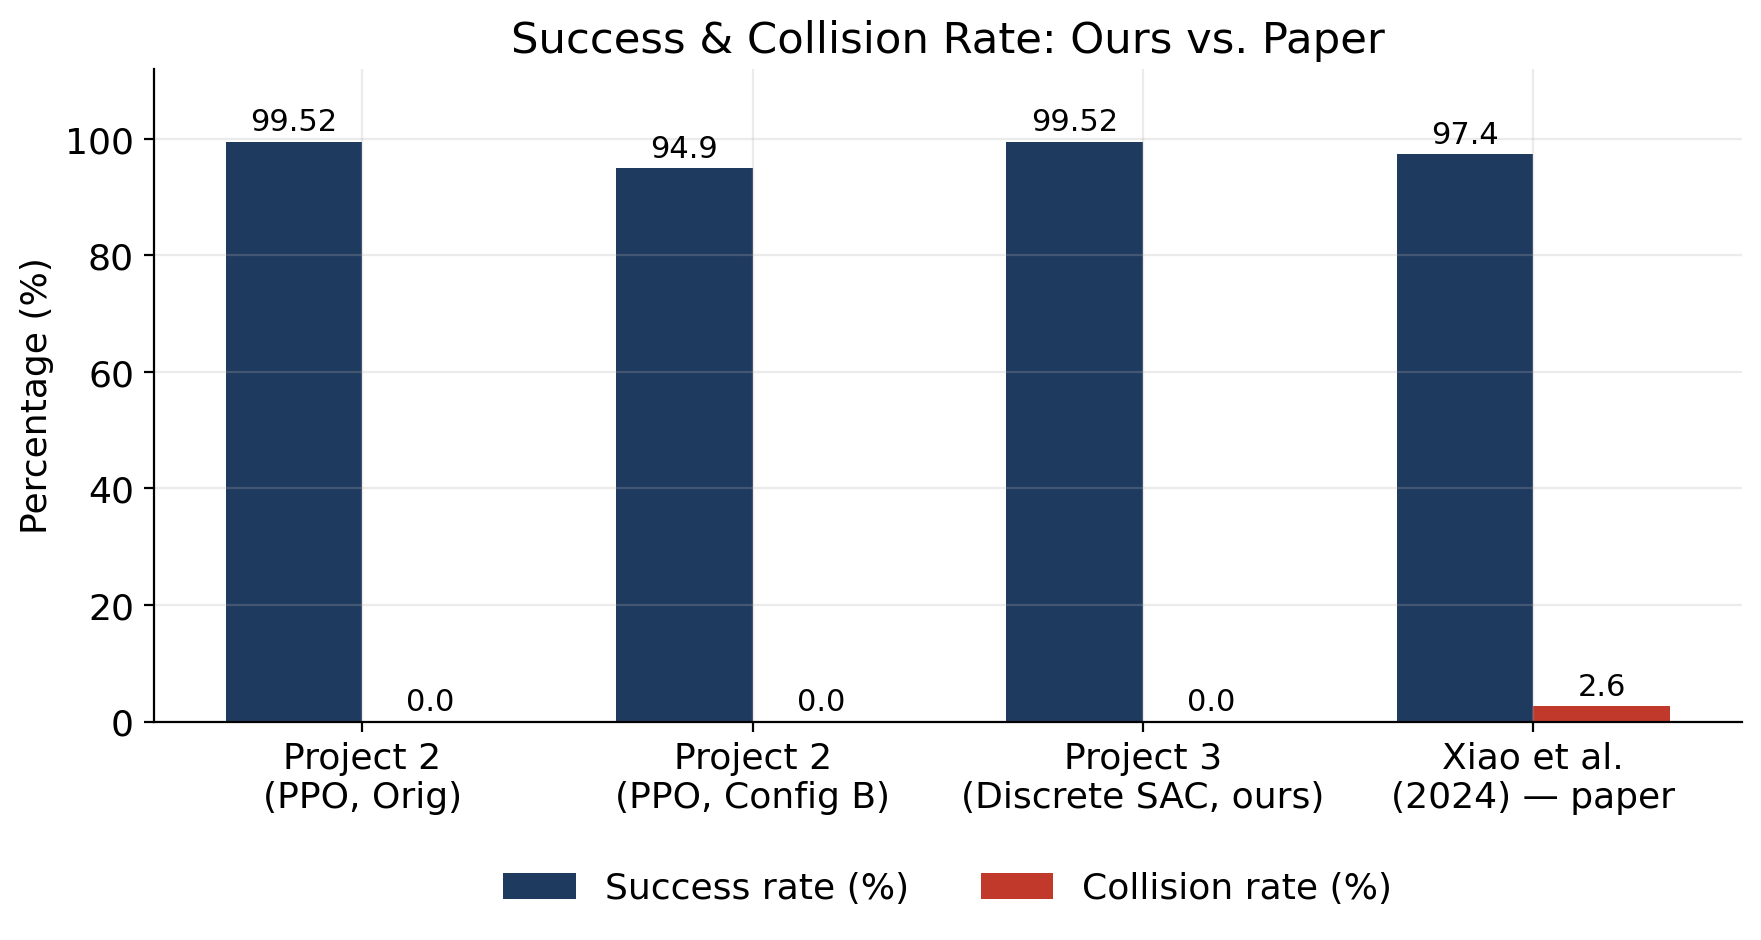
\includegraphics[width=0.60\linewidth]{img/success_collision_chart.png}\\[8pt]
	\small 99.52\% success, 0\% collisions over 1{,}050 episodes --- exceeds the paper's 97.4\%/2.6\%.
\end{frame}

\begin{frame}{Result 2: Mean Crossing Speed}
	\centering
	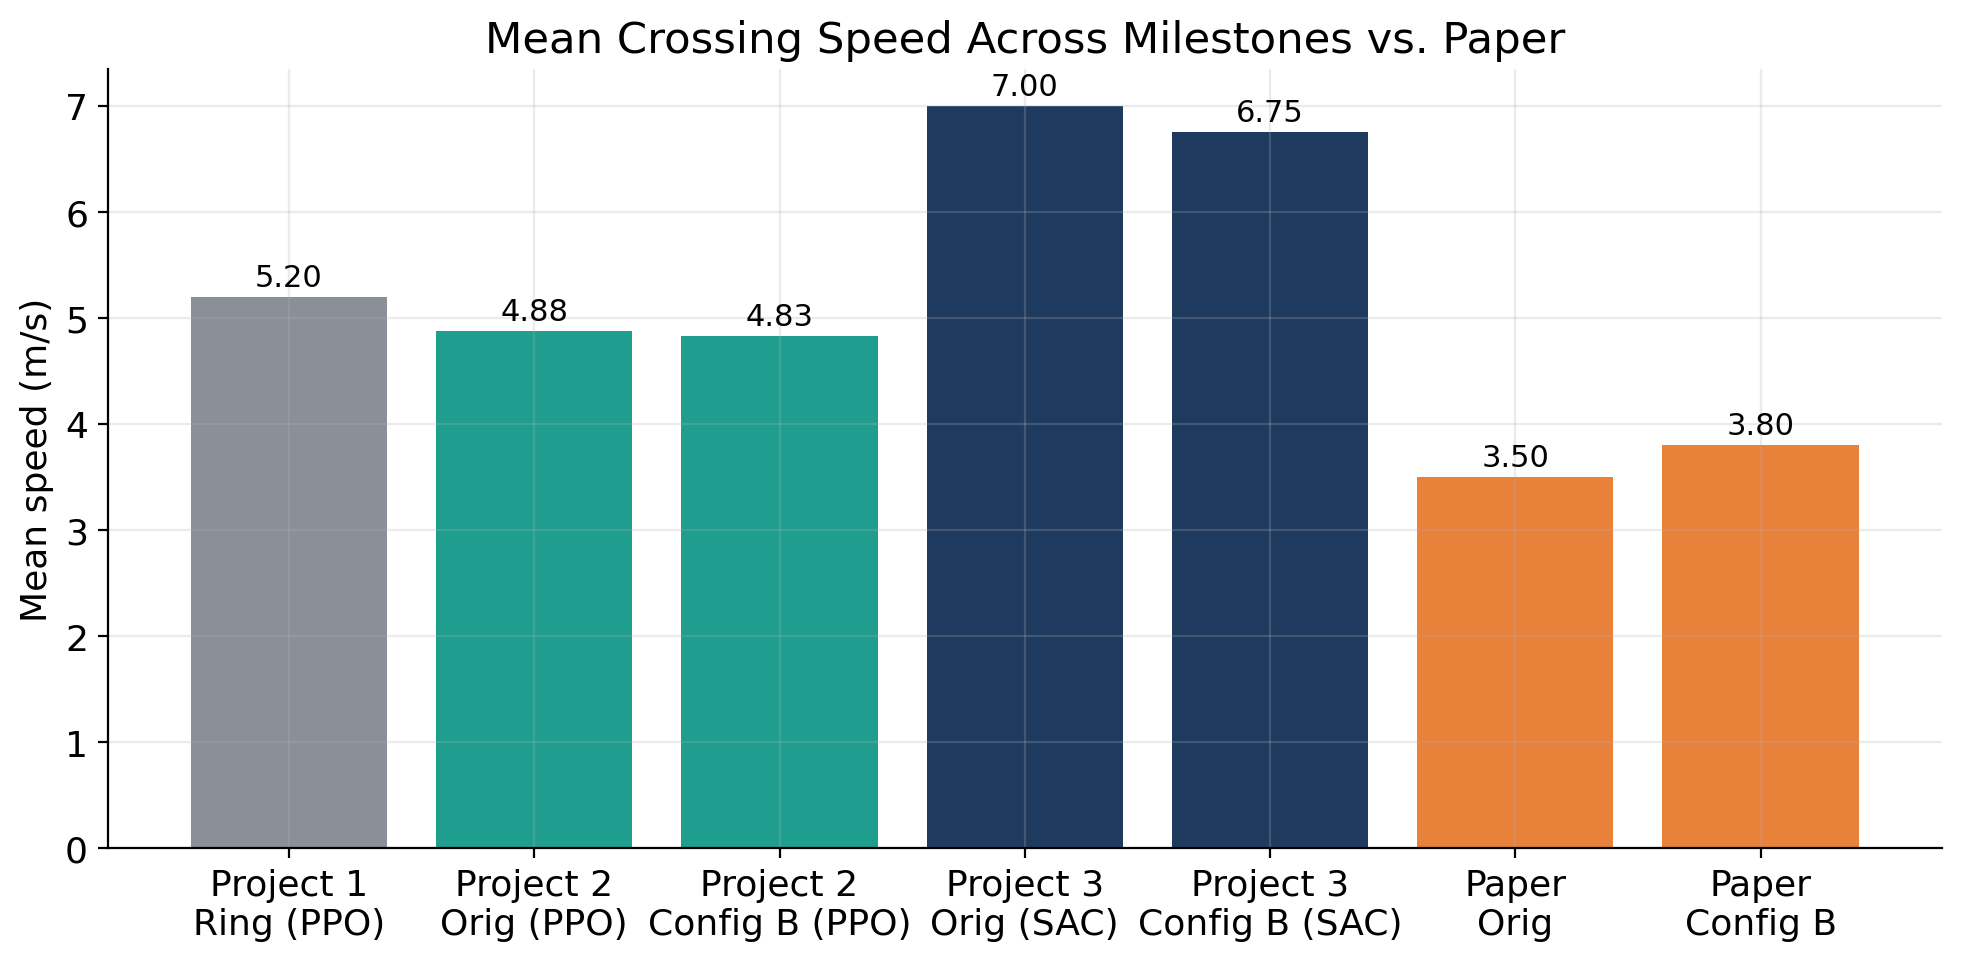
\includegraphics[width=0.66\linewidth]{img/speed_comparison_chart.png}\\[8pt]
	\small Nearly \textbf{2$\times$ faster} crossing than the paper --- the simulators are not physically equivalent.
\end{frame}

\begin{frame}{Result 3: Intent-Driven Speed Modulation}
	\centering
	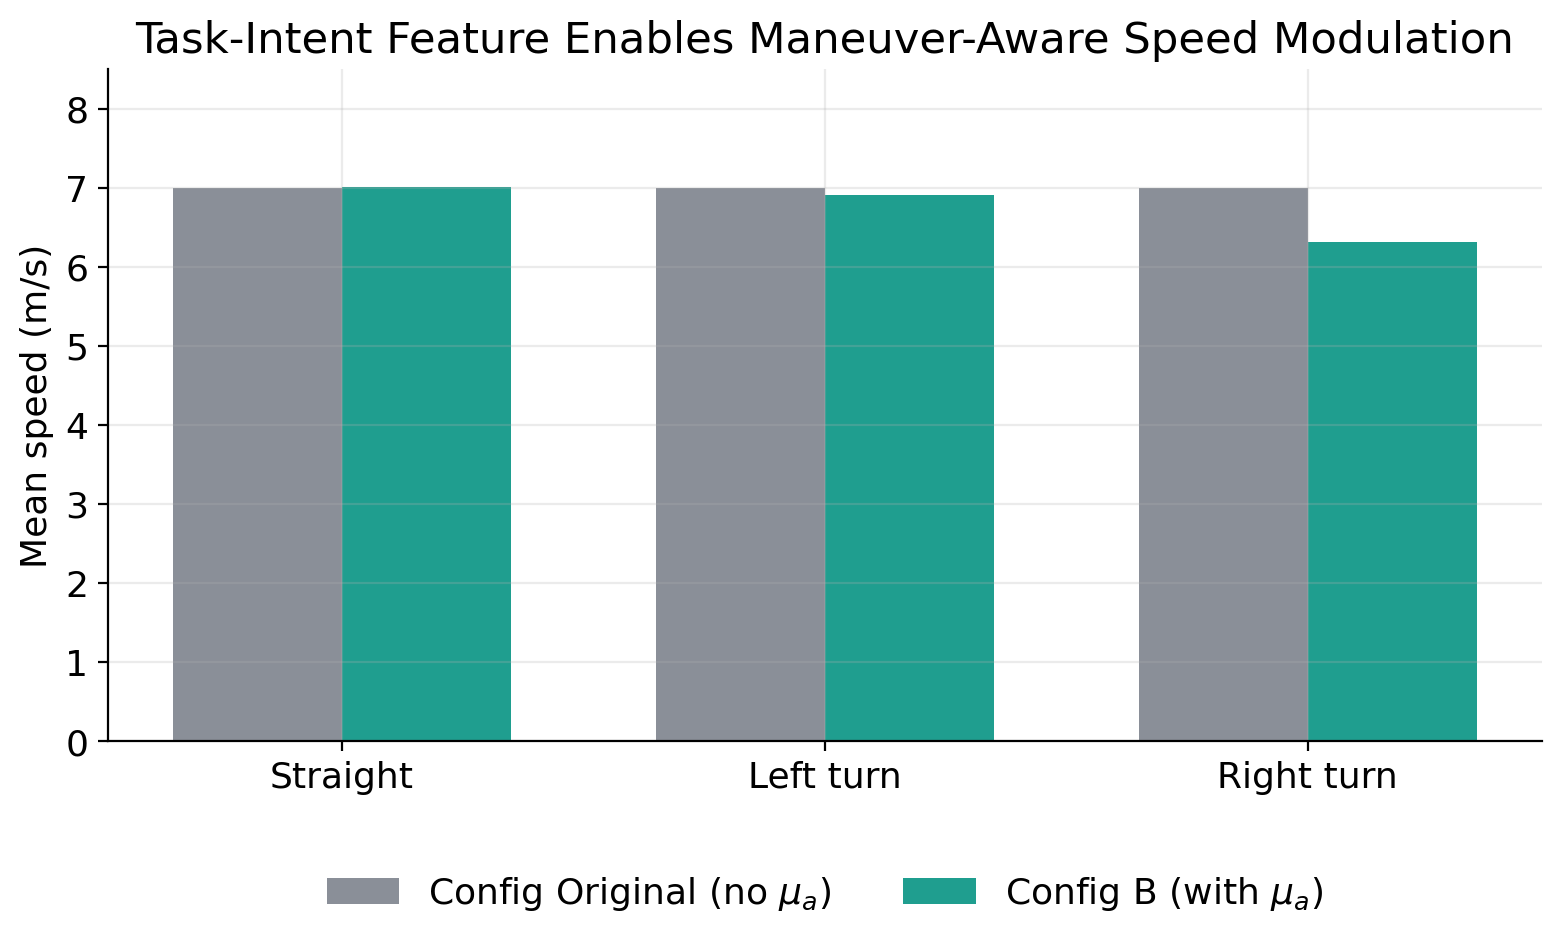
\includegraphics[width=0.54\linewidth]{img/intent_speed_modulation.png}\\[8pt]
	\small Config B ($+\mu_a$) slows for turns (Left 6.91, Right 6.32 m/s); Original stays uniform ($\sim$7.00 m/s).
\end{frame}


% =====================================================================
\section{Challenges and Limitations}
% =====================================================================

\begin{frame}{Challenges and Limitations}
	\begin{columns}[T]
		\begin{column}{0.48\textwidth}
			\begin{block}{Incomplete Paper Specification}
				\small Unreleased paper constants \& parameters recovered via systematic inference.
			\end{block}
		\end{column}
		\begin{column}{0.48\textwidth}
			\begin{block}{Non-Generalizable Baseline Policy}
				\small Current reproduction is a traditional baseline; lacks geometry invariance and cannot transfer.
			\end{block}
		\end{column}
	\end{columns}
	\vspace{10pt}
	\begin{columns}[T]
		\begin{column}{0.48\textwidth}
			\begin{block}{Sim-to-Sim Kinematics Divergence}
				\small Micro-yielding behavior and collision physics differ between \texttt{highway-env} and paper sim.
			\end{block}
		\end{column}
		\begin{column}{0.48\textwidth}
			\begin{block}{Single Fixed Geometry Overfitting}
				\small Policy is overfit to a standard 4-way cross; fails on T-junctions, merges, or roundabouts.
			\end{block}
		\end{column}
	\end{columns}
\end{frame}

% =====================================================================
\section{Conclusion and Future Direction}
% =====================================================================

\begin{frame}{Next Semester Focus: Generalizable Decision-Making}
	\begin{alertblock}{Core Limitation of Current Work}
		\small The reproduced Discrete SAC model is a \textbf{traditional single-geometry policy} tied to one 4-way layout. Real-world autonomous driving requires handling arbitrary junction topologies.
	\end{alertblock}
	\vspace{8pt}
	\textbf{Thesis Objective (Next Semester):} Develop a truly geometry-agnostic decision policy.
	\begin{itemize}\setlength{\itemsep}{5pt}
		\item \textbf{Invariant State Representation:} Replace fixed coordinates with conflict graphs and relative TTC
		\item \textbf{Cross-Topology Evaluation:} Zero-shot and few-shot transfer to T-junctions, roundabouts, and merges
		\item \textbf{Generalization Metric:} Quantify transfer of right-of-way negotiation without per-scenario retraining
	\end{itemize}
\end{frame}

\begin{frame}{Generalization Strategy}
	\centering
	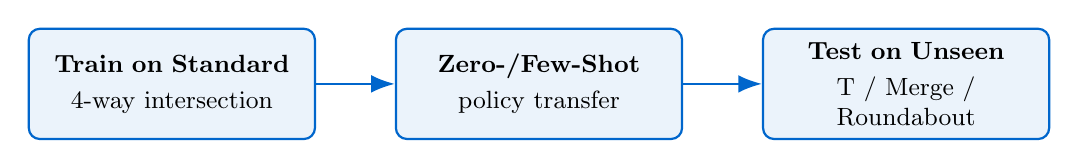
\begin{tikzpicture}[
			node distance=10mm and 10mm,
			every node/.style={font=\small},
			block/.style={draw=accentblue, thick, rounded corners, fill=accentblue!8, minimum height=1.4cm, text width=3.4cm, align=center},
			arrowstyle/.style={-{Latex[length=3mm]}, thick, accentblue}
		]
		\node[block] (train) {\textbf{Train on Standard}\\[2pt] 4-way intersection};
		\node[block, right=of train] (transfer) {\textbf{Zero-/Few-Shot}\\[2pt] policy transfer};
		\node[block, right=of transfer] (test) {\textbf{Test on Unseen}\\[2pt] T / Merge / Roundabout};
		\draw[arrowstyle] (train) -- (transfer);
		\draw[arrowstyle] (transfer) -- (test);
	\end{tikzpicture}
	\vspace{16pt}

	\small Graph-based and relational representations generalize far better across unseen junction layouts than fixed-coordinate vectors.
\end{frame}

\begin{frame}{Proposed Project Timeline}
	\centering
	\resizebox{0.96\textwidth}{!}{%
		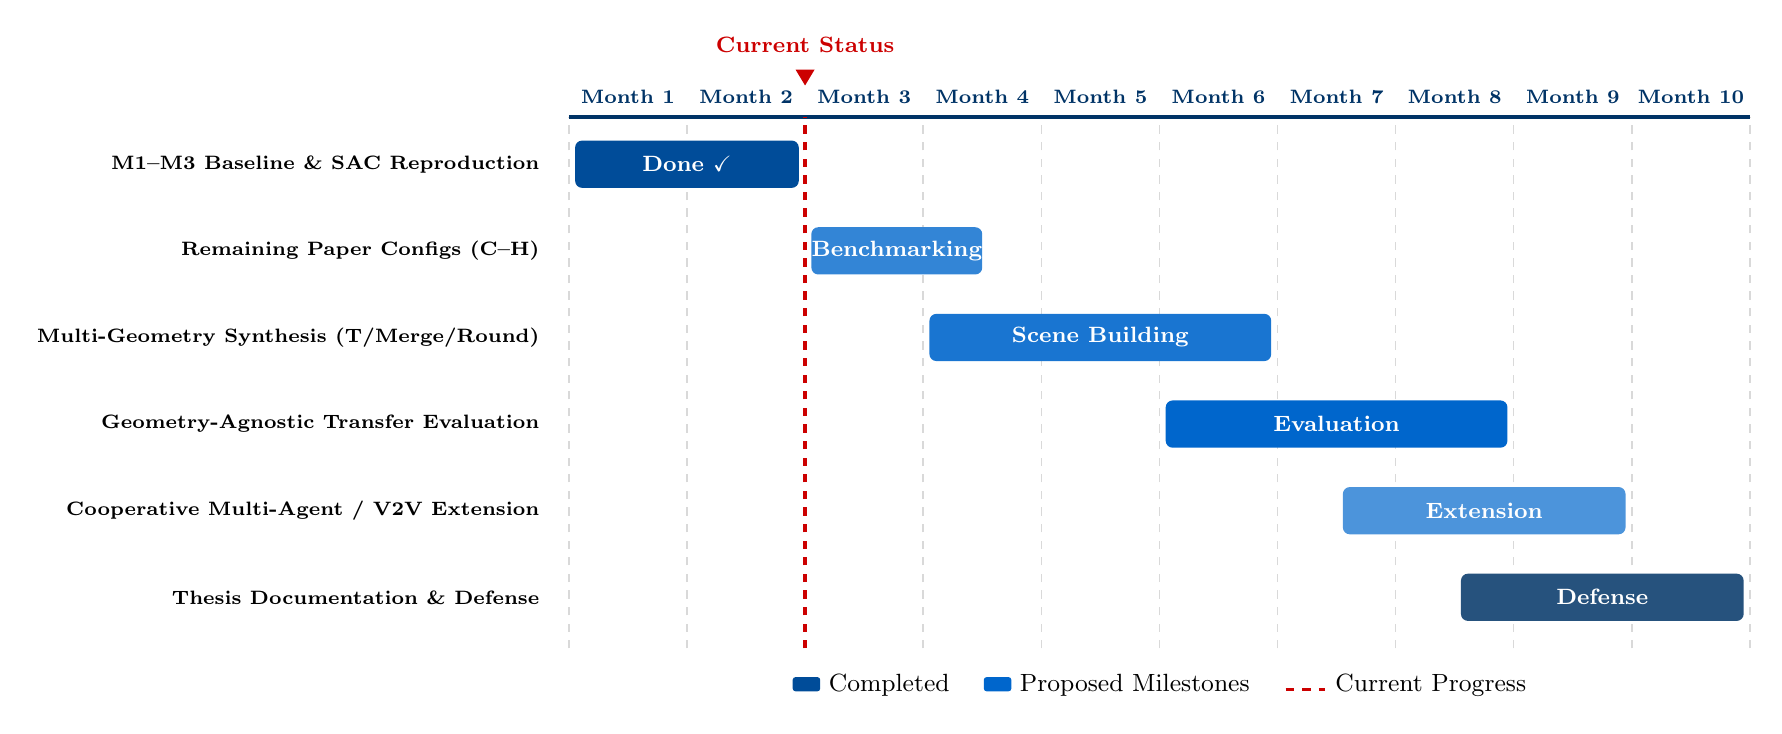
\begin{tikzpicture}[
				task/.style={font=\scriptsize\bfseries, anchor=east, align=right},
				bar/.style={rounded corners=2.5pt, minimum height=0.42cm},
				gridline/.style={draw=gray!30, dashed, line width=0.5pt},
				monthhdr/.style={font=\scriptsize\bfseries, text=mainblue, anchor=south}
			]
			\foreach \m [count=\i from 0] in {Month 1, Month 2, Month 3, Month 4, Month 5, Month 6, Month 7, Month 8, Month 9, Month 10} {
					\node[monthhdr] at (\i*1.5 + 0.75, 3.4) {\m};
					\draw[gridline] (\i*1.5, -3.4) -- (\i*1.5, 3.35);
				}
			\draw[gridline] (15.0, -3.4) -- (15.0, 3.35);
			\draw[draw=mainblue, line width=1.5pt] (0, 3.35) -- (15.0, 3.35);

			% Task 1
			\node[task] at (-0.25, 2.75) {M1--M3 Baseline \& SAC Reproduction};
			\fill[blockheaderblue, bar] (0.08, 2.45) rectangle (2.92, 3.05) node[midway, font=\footnotesize\bfseries, text=white] {Done \checkmark};

			% Task 2
			\node[task] at (-0.25, 1.65) {Remaining Paper Configs (C--H)};
			\fill[accentblue!80, bar] (3.08, 1.35) rectangle (5.25, 1.95) node[midway, font=\footnotesize\bfseries, text=white] {Benchmarking};

			% Task 3
			\node[task] at (-0.25, 0.55) {Multi-Geometry Synthesis (T/Merge/Round)};
			\fill[accentblue!90, bar] (4.58, 0.25) rectangle (8.92, 0.85) node[midway, font=\footnotesize\bfseries, text=white] {Scene Building};

			% Task 4
			\node[task] at (-0.25, -0.55) {Geometry-Agnostic Transfer Evaluation};
			\fill[accentblue, bar] (7.58, -0.85) rectangle (11.92, -0.25) node[midway, font=\footnotesize\bfseries, text=white] {Evaluation};

			% Task 5
			\node[task] at (-0.25, -1.65) {Cooperative Multi-Agent / V2V Extension};
			\fill[accentblue!70, bar] (9.83, -1.95) rectangle (13.42, -1.35) node[midway, font=\footnotesize\bfseries, text=white] {Extension};

			% Task 6
			\node[task] at (-0.25, -2.75) {Thesis Documentation \& Defense};
			\fill[mainblue!85, bar] (11.33, -3.05) rectangle (14.92, -2.45) node[midway, font=\footnotesize\bfseries, text=white] {Defense};

			% Current Timeline Marker (after Month 2, exactly 8 months remaining)
			\draw[draw=red!80!black, line width=1.4pt, dashed] (3.0, -3.4) -- (3.0, 3.35);
			\fill[red!80!black] (2.88, 3.95) -- (3.12, 3.95) -- (3.0, 3.75) -- cycle;
			\node[font=\footnotesize\bfseries, text=red!80!black, anchor=south] at (3.0, 4.05) {Current Status};

			% Legend
			\node[anchor=north, font=\small] at (7.5, -3.6) {
				\tikz\fill[blockheaderblue, rounded corners=1pt] (0,0) rectangle (0.35, 0.18); Completed \quad
				\tikz\fill[accentblue, rounded corners=1pt] (0,0) rectangle (0.35, 0.18); Proposed Milestones \quad
				\tikz\draw[red!80!black, line width=1.3pt, dashed] (0,0) -- (0.5, 0); Current Progress
			};
		\end{tikzpicture}%
	}
\end{frame}

\begin{frame}{Conclusion}
	\begin{itemize}\setlength{\itemsep}{7pt}
		\item \textbf{Completed Milestone (Current Semester):} Rigorous 1:1 reproduction of the published \alert{traditional RL baseline} (Discrete SAC, 99.52\% success, 0\% collisions over 1{,}050 tests).
		\item \textbf{Root-Cause Insights:} Identified simulator micro-yielding physics divergence and eliminated hybrid-CPU bottlenecks ($3.5\times$ throughput speedup).
		\item \textbf{Foundational Limitation:} Firmly established that traditional coordinate-based RL is \alert{not generalizable} across intersection topologies.
		\item \textbf{Next Semester Thesis Research:} Formulated the concrete architecture and roadmap for \textbf{Generalizable, Geometry-Agnostic Decision-Making}.
	\end{itemize}
\end{frame}

% =====================================================================
\section{Project Repository}
% =====================================================================

\begin{frame}{GitHub Contributors Activity Graph}
	\centering
	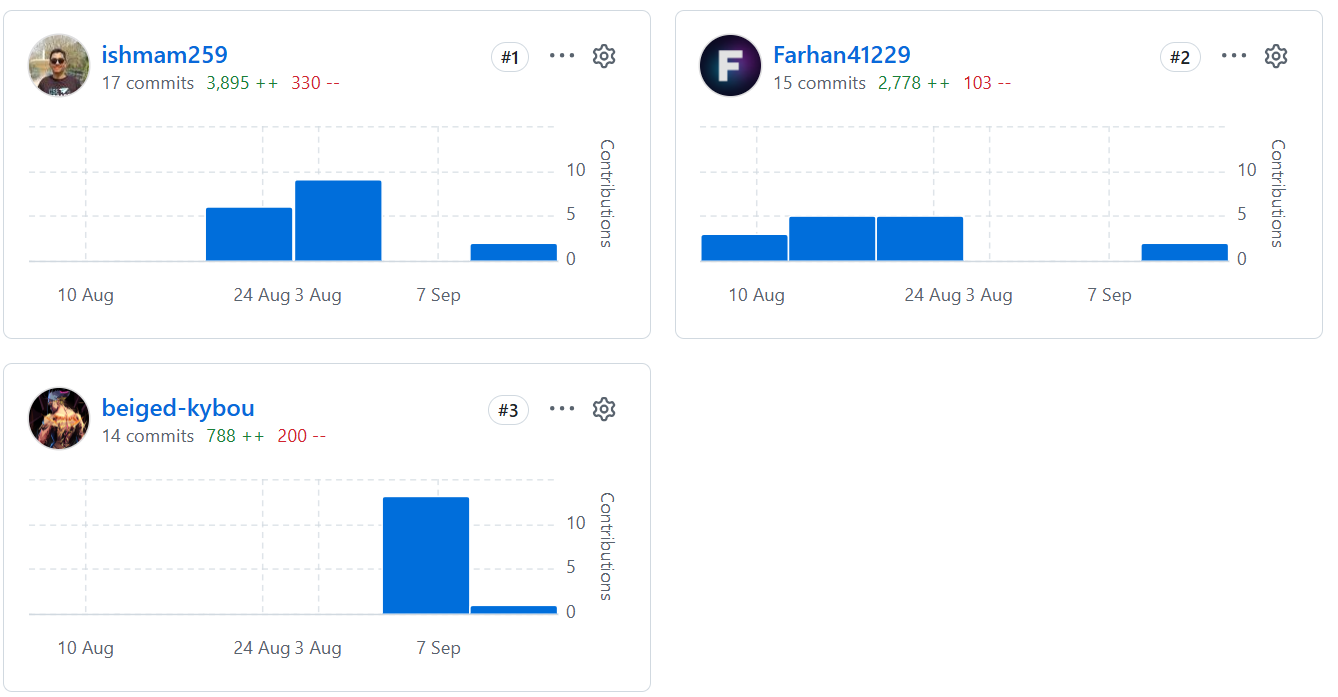
\includegraphics[height=0.82\textheight, keepaspectratio]{c.png}
\end{frame}

\begin{frame}
	\centering
	\vspace{10pt}
	{\Huge \textbf{\color{navy}Thank You!}}\\[16pt]
	{\Large \textbf{\color{accentblue}Questions \& Discussion}}\\[24pt]
	\begin{block}{Project Repository}
		\centering \small \url{https://github.com/Farhan41229/Drl-unsignalized-intersection-navigation}
	\end{block}
\end{frame}

% =====================================================================
\appendix
\begin{frame}[allowframebreaks]{References}
	\tiny
	\nocite{*}
	\bibliographystyle{plain}
	\bibliography{references}
\end{frame}

\end{document}
